% !TEX root = ./main.tex

\documentclass[conference]{IEEEtran}

\IEEEoverridecommandlockouts

\usepackage{cite}

\usepackage{amsmath,amssymb,amsfonts}

\usepackage{algorithmic}

\usepackage{algorithm}

\usepackage{graphicx}

\graphicspath{{figures/}}

\usepackage{textcomp}

\usepackage{xcolor}

\usepackage{tikz}

\usetikzlibrary{shapes.geometric,arrows.meta,positioning,fit,backgrounds,calc,shadows}

\usepackage{booktabs}

\usepackage{array}

\usepackage{url}

\usepackage{microtype}

\usepackage{balance}

\def\BibTeX{{\rm B\kern-.05em{\sc i\kern-.025em b}\kern-.08em

    T\kern-.1667em\lower.7ex\hbox{E}\kern-.125emX}}

% === ICON MACROS ===

\newcommand{\icDB}[3]{\begin{scope}[shift={(#1,#2)},scale=#3]

\draw[fill=teal!18,draw=teal!70!black,line width=0.8pt] (-0.42,0.34) -- (-0.42,-0.34) arc (180:360:0.42 and 0.14) -- (0.42,0.34) -- cycle;

\draw[teal!70!black,line width=0.6pt] (-0.42,0.06) arc (180:360:0.42 and 0.14);

\draw[teal!70!black,line width=0.6pt] (-0.42,-0.14) arc (180:360:0.42 and 0.14);

\draw[fill=teal!40,draw=teal!70!black,line width=0.8pt] (0,0.34) ellipse (0.42 and 0.14);

\end{scope}}

\newcommand{\icScreen}[3]{\begin{scope}[shift={(#1,#2)},scale=#3]

\draw[rounded corners=2pt,fill=black!75,draw=black!85,line width=0.8pt] (-0.62,-0.42) rectangle (0.62,0.42);

\fill[white] (-0.53,-0.33) rectangle (0.53,0.33);

\fill[green!55!black] (-0.3,0.12) circle (0.08); \fill[blue!65!black] (0,0.12) circle (0.08); \fill[red!70!black] (0.3,0.12) circle (0.08);

\draw[black!35,line width=0.7pt] (-0.38,-0.12)--(0.38,-0.12); \draw[black!25,line width=0.7pt] (-0.38,-0.24)--(0.2,-0.24);

\fill[black!70] (-0.1,-0.42) rectangle (0.1,-0.54); \fill[black!70] (-0.3,-0.6) rectangle (0.3,-0.52);

\end{scope}}

\newcommand{\icPerson}[4]{\begin{scope}[shift={(#1,#2)},scale=#3]

\fill[#4] (0,0.3) circle (0.18);

\fill[#4] (-0.34,-0.42) .. controls (-0.34,0.06) and (0.34,0.06) .. (0.34,-0.42) -- cycle;

\end{scope}}

\newcommand{\icDoctor}[3]{\icPerson{#1}{#2}{#3}{red!60!black}\begin{scope}[shift={(#1,#2)},scale=#3]

\fill[white] (-0.04,-0.28) rectangle (0.04,-0.06); \fill[white] (-0.13,-0.19) rectangle (0.13,-0.11);

\end{scope}}

\newcommand{\icServer}[3]{\begin{scope}[shift={(#1,#2)},scale=#3]

\foreach \yy in {0.34,0,-0.34}{\draw[rounded corners=1.5pt,fill=blue!12,draw=blue!60!black,line width=0.8pt] (-0.5,\yy-0.14) rectangle (0.5,\yy+0.14);

\fill[green!55!black] (-0.36,\yy) circle (0.045); \fill[blue!60!black] (-0.22,\yy) circle (0.045); \draw[blue!50!black,line width=0.6pt] (0.02,\yy)--(0.38,\yy);}

\end{scope}}

\newcommand{\icGear}[3]{\begin{scope}[shift={(#1,#2)},scale=#3]

\node[star,star points=9,star point ratio=0.82,draw=orange!80!black,fill=orange!30,line width=0.8pt,minimum size=0.95cm,inner sep=0pt] at (0,0) {};

\fill[white] (0,0) circle (0.15); \draw[orange!80!black,line width=0.6pt] (0,0) circle (0.15);

\end{scope}}

\newcommand{\icMagnifier}[3]{\begin{scope}[shift={(#1,#2)},scale=#3]

\draw[line width=2.4pt,draw=blue!60!black,line cap=round] (0.2,-0.2)--(0.5,-0.5);

\draw[fill=blue!8,draw=blue!60!black,line width=1.4pt] (-0.08,0.08) circle (0.34);

\node[font=\scriptsize,text=blue!60!black] at (-0.08,0.08) {$\Sigma$};

\end{scope}}

\newcommand{\icNet}[3]{\begin{scope}[shift={(#1,#2)},scale=#3]

\draw[purple!60!black,line width=0.9pt] (-0.4,0.25)--(0,-0.3)--(0.4,0.25) (-0.4,0.25)--(0.4,0.25) (0,-0.3)--(0,0.45);

\foreach \px/\py in {-0.4/0.25,0.4/0.25,0/-0.3,0/0.45}{\draw[fill=purple!25,draw=purple!60!black,line width=0.8pt] (\px,\py) circle (0.1);}

\end{scope}}

\newcommand{\icShield}[3]{\begin{scope}[shift={(#1,#2)},scale=#3]

\draw[fill=green!20,draw=green!45!black,line width=1pt] (0,0.5) .. controls (0.22,0.42) and (0.4,0.4) .. (0.4,0.3) -- (0.4,-0.02) .. controls (0.4,-0.3) and (0.15,-0.45) .. (0,-0.55) .. controls (-0.15,-0.45) and (-0.4,-0.3) .. (-0.4,-0.02) -- (-0.4,0.3) .. controls (-0.4,0.4) and (-0.22,0.42) .. cycle;

\draw[green!40!black,line width=1.8pt,line cap=round,line join=round] (-0.17,0) -- (-0.04,-0.14) -- (0.2,0.18);

\end{scope}}

\newcommand{\icImage}[3]{\begin{scope}[shift={(#1,#2)},scale=#3]

\draw[rounded corners=2pt,fill=gray!12,draw=black!55,line width=0.8pt] (-0.55,-0.42) rectangle (0.55,0.42);

\fill[gray!55] (-0.45,-0.34) -- (-0.15,0.05) -- (0.05,-0.18) -- (0.25,0.08) -- (0.45,-0.34) -- cycle;

\fill[gray!45] (0.28,0.2) circle (0.09);

\end{scope}}

\begin{document}

\title{Auditing Machine Learning in Autism Screening: From Rule Rediscovery to Adaptive Triage}

\author{

\begin{tabular}[t]{c@{\hskip 0.02\textwidth}c@{\hskip 0.02\textwidth}c}

\begin{minipage}[t]{0.30\textwidth}\centering

1\textsuperscript{st} Kantam Gowri\\

\textit{Dept. of Computer Science and Engineering}\\

\textit{Vel Tech Rangarajan Dr. Sagunthala}\\

\textit{R\&D Institute of Science and Technology}\\

Chennai, Tamil Nadu, India\\

Vtu24895@veltech.edu.in

\end{minipage}

&

\begin{minipage}[t]{0.30\textwidth}\centering

2\textsuperscript{nd} Rekhana Jayavardhan Rao\\

\textit{Dept. of Computer Science and Engineering}\\

\textit{Vel Tech Rangarajan Dr. Sagunthala}\\

\textit{R\&D Institute of Science and Technology}\\

Chennai, Tamil Nadu, India\\

Vtu25063@veltech.edu.in

\end{minipage}

&

\begin{minipage}[t]{0.30\textwidth}\centering

3\textsuperscript{rd} Prathik A\\

\textit{Assistant Professor}\\

\textit{Dept. of Computer Science and Engineering}\\

\textit{Vel Tech Rangarajan Dr. Sagunthala}\\

\textit{R\&D Institute of Science and Technology}\\

Chennai, Tamil Nadu, India\\

prathik0505@gmail.com

\end{minipage}

\end{tabular}

}

\maketitle

\begin{abstract}
Published research consistently notes 98\%--100\% assessment of machine learning diagnostic accuracy using public automated autism screening collections and childhood facial images. Our empirical audit reveals these metrics stem from benchmark design artifacts rather than clinical discovery. For four cohorts of publicly available behavioral survey samples ($N=2{,}154$), the target label is an unweighted integer sum threshold over 10 responses ($t = 4$ for toddlers; $t = 7$ for older groups); top classifiers rely on reconstructing this arithmetic addition rule. Training only on background demographics and family history gives only weak to moderate signal (raw ROC-AUC between 0.56 and 0.72, balanced accuracy ranging from 50\% to 61\%).

On the open pediatric facial image benchmark (3,014 photographs), systematic capture bias takes the lead in class separation: automated quality filters accept only 16.32\% of autistic subjects vs 29.99\% of controls ($p = 5.44 \times 10^{-19}$). Grad-CAM saliency mass captures 51.73\% of attribution energy on the outer 10\% of the image border (more than the 36.00\% geometric baseline), confirming that computer vision backbones exploit photo framing shortcuts.

Revising computational tools for adaptive clinical triage: Sequential questions ordered by conditional mutual information reduce questionnaire length by 31.4\% to 53.8\% (mean 4.62 to 6.86 items per test) with minimum 95.07\% agreement to the complete instruments. Lastly, split-conformal prediction provides marginal coverage under exchangeability (mean observed coverage 95.4--96.7\% over 100 splits at the 0.05 level), substituting forced binary classification with automated specialist referral on uncertain cases.
\end{abstract}

\begin{IEEEkeywords}
Autism Spectrum Disorder, Dataset Leakage, Algorithmic Audit, Conformal Prediction, Adaptive Screening.
\end{IEEEkeywords}

\section{Introduction}

Autism Spectrum Disorder (ASD) involves atypical developmental trajectories in reciprocal communication, social engagement, and repetitive behaviors~\cite{american2013diagnostic}. In the past decade, there has been a growing literature in computer science that has applied supervised classifiers to public screening surveys, reporting repeated cross-validation accuracies of 98\% to 100\%~\cite{thabtah2019machine}. At the same time, a number of publications claim that deep convolutional networks are capable to detect autism in children based only on snapshot facial photographs. These claims contradict basic clinical facts, and are presented as breakthroughs in automated health care. Psychometricians have developed short screening tools such as the 10-item Autism Spectrum Quotient (AQ-10) and the Quantitative Checklist in Toddlers (Q-CHAT-10) as initial triage scales scored by simple integer summing~\cite{allison2012toward}. Using a machine learning classifier to predict an outcome that is itself defined by summing those same questions does not reveal interactive finer-grained behavior; it simply draws a decision boundary around a linear arithmetic sum. Meanwhile, training deep vision models with high capacity from photographs of children in uncontrolled environments is susceptible to picking up background artifacts, changes in lighting, and camera vignetting rather than facial shape~\cite{geirhos2020shortcut}.

The work describes a formal reproducibility audit of publicly available screening datasets, and a practical computational triage pipeline as shown in Fig.~\ref{fig:architecture}:

\begin{enumerate}
    \item \textbf{rediscovery of deterministic rules}: We demonstrate that target labels in all four standard cohorts ($N = 2{,}154$) are exact step functions over survey responses ($t = 4$ in toddlers; $t = 7$ in children, adolescents, and adults).
    \item \textbf{Limited Demographic Signal}: Classifiers trained on demographics and family history alone are weak to modest in signal (raw ROC-AUC 0.56--0.72, balanced accuracy 50--61\%), indicating that demographic markers cannot replace behavioural observation.
    \item \textbf{Constructive Reformulation}: Rather than seeking superfluous diagnostic labels, the value of machine learning lies in reducing the length of questionnaires while preserving scoring fidelity.
    \item \textbf{Adaptive Bayesian Stopping}: We sequentially rank items by conditional mutual information with our dynamic questioner to reduce response burden by 31.4\% to 53.8\% while achieving $\ge 95.07\%$ agreement.
    \item \textbf{Conformal Risk Abstention}: Through split-conformal calibration on held-out data, our screener delivers marginal coverage under exchangeability, deferring borderline profiles for specialist evaluation.
    \item \textbf{Facial Benchmark Audit}: An exhaustive audit of the 3,014 pediatric photos in the Kaggle benchmark exposes sharp acquisition disparities and peripheral border artifacts, demonstrating why image models should not be used in autism triage.
\end{enumerate}

\begin{figure*}[!t]

\centering

\resizebox{0.96\textwidth}{!}{
%
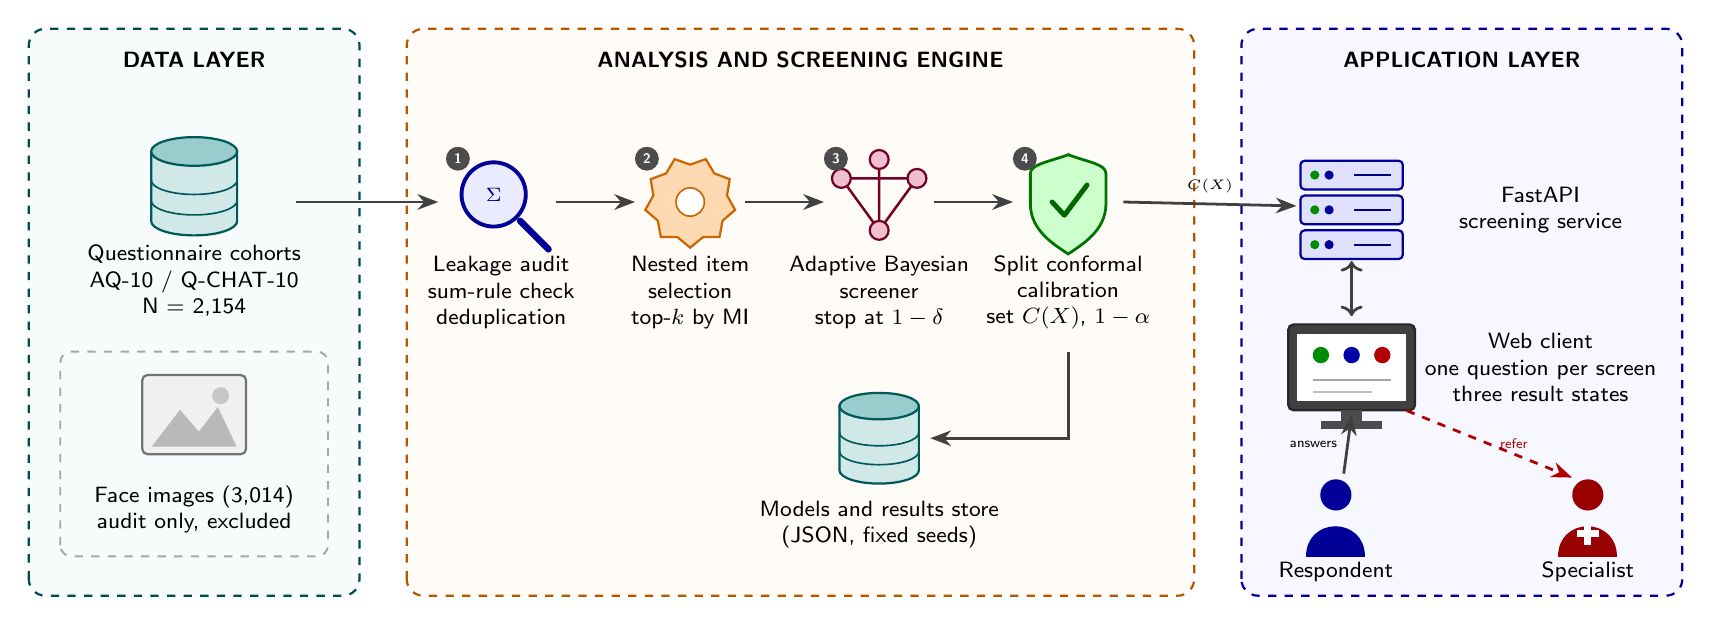
\begin{tikzpicture}[
lab/.style={font=\footnotesize\sffamily,text centered,align=center,inner sep=1pt},
labb/.style={lab,font=\footnotesize\bfseries\sffamily},
badge/.style={circle,fill=black!70,text=white,font=\tiny\bfseries\sffamily,inner sep=1.5pt},
arr/.style={-{Stealth[scale=1.0]},line width=1.0pt,draw=black!75},
darr/.style={-{Stealth[scale=1.0]},dashed,line width=1.0pt,draw=red!70!black},
panel/.style={dashed,rounded corners=6pt,line width=0.8pt}]
\draw[panel,draw=teal!60!black,fill=teal!3] (0,0) rectangle (4.2,7.2);
\node[labb] at (2.1,6.8) {DATA LAYER};
\draw[panel,draw=orange!70!black,fill=orange!3] (4.8,0) rectangle (14.8,7.2);
\node[labb] at (9.8,6.8) {ANALYSIS AND SCREENING ENGINE};
\draw[panel,draw=blue!60!black,fill=blue!3] (15.4,0) rectangle (21.0,7.2);
\node[labb] at (18.2,6.8) {APPLICATION LAYER};
\icDB{2.1}{5.2}{1.3}
\node[lab] at (2.1,4.0) {Questionnaire cohorts\\AQ-10 / Q-CHAT-10\\N = 2,154};
\draw[dashed,gray!70,rounded corners=4pt,line width=0.7pt] (0.4,0.5) rectangle (3.8,3.1);
\icImage{2.1}{2.3}{1.2}
\node[lab] at (2.1,1.1) {Face images (3,014)\\audit only, excluded};
\icMagnifier{6.0}{5.0}{1.2}\node[badge] at (5.45,5.55) {1};
\node[lab] at (6.0,3.85) {Leakage audit\\sum-rule check\\deduplication};
\icGear{8.4}{5.0}{1.2}\node[badge] at (7.85,5.55) {2};
\node[lab] at (8.4,3.85) {Nested item\\selection\\top-$k$ by MI};
\icNet{10.8}{5.0}{1.2}\node[badge] at (10.25,5.55) {3};
\node[lab] at (10.8,3.85) {Adaptive Bayesian\\screener\\stop at $1-\delta$};
\icShield{13.2}{5.0}{1.2}\node[badge] at (12.65,5.55) {4};
\node[lab] at (13.2,3.85) {Split conformal\\calibration\\set $C(X)$, $1-\alpha$};
\draw[arr] (3.4,5.0)--(5.2,5.0);
\draw[arr] (6.7,5.0)--(7.7,5.0);
\draw[arr] (9.1,5.0)--(10.1,5.0);
\draw[arr] (11.5,5.0)--(12.5,5.0);
\icDB{10.8}{2.0}{1.2}
\node[lab] at (10.8,0.9) {Models and results store\\(JSON, fixed seeds)};
\draw[arr] (13.2,3.1)|-(11.45,2.0);
\icServer{16.8}{4.9}{1.3}\node[lab] at (19.2,4.9) {FastAPI\\screening service};
\icScreen{16.8}{2.9}{1.3}\node[lab] at (19.2,2.9) {Web client\\one question per screen\\three result states};
\icPerson{16.6}{0.95}{1.1}{blue!60!black}\node[lab] at (16.6,0.3) {Respondent};
\icDoctor{19.8}{0.95}{1.1}\node[lab] at (19.8,0.3) {Specialist};
\draw[arr] (13.9,5.0)--(16.1,4.95) node[midway,above,font=\tiny\sffamily] {$C(X)$};
\draw[arr,<->] (16.8,4.25)--(16.8,3.55);
\draw[arr] (16.7,1.55)--(16.8,2.3) node[midway,left,font=\tiny\sffamily] {answers};
\draw[darr] (17.5,2.35)--(19.6,1.5) node[midway,right,font=\tiny\sffamily,text=red!70!black] {refer};
\end{tikzpicture}
}

\caption{System architecture of the proposed framework: data layer (public questionnaire cohorts and an exploratory face-image set that is excluded from screening decisions), analysis engine (leakage audit, nested item selection, adaptive Bayesian screener, and split conformal calibration) and application layer (FastAPI service, web client, respondent and specialist referral).}

\label{fig:architecture}

\end{figure*}

\section{Related Work}

\noindent\textbf{Clinical Foundations and Psychometric Rubrics}:
Under DSM-5 criteria, ASD diagnosis is made through a multidisciplinary assessment of reciprocal communication as well as restricted, repetitious actions~\cite{american2013diagnostic}. Allison and colleagues created the brief AQ-10 and toddler Q-CHAT-10 to offer primary care a fast triage tool~\cite{allison2012toward}. Both scales use straightforward, unweighted scoring cutoffs to assist clinicians in determining whether to refer a child to a specialist; neither instrument was ever created for a stand-alone, independent diagnosis.

\noindent\textbf{Supervised Classification and Questionnaire Repositories}:
Thabtah suggested frameworks for machine learning adaptation under DSM-5 standards~\cite{thabtah2017autism} and computational feature analysis methods~\cite{thabtah2018qchat} with datasets located on the UCI Machine Learning Repository for adults, children, and adolescents~\cite{uci_asd_adult, uci_asd_child, uci_asd_adolescent} and on Kaggle for toddlers~\cite{kaggle_toddler}. Subsequent computer science papers applied various machine learning pipelines to these records, repeatedly reporting near-perfect classification rates~\cite{thabtah2019machine}. Many of these works used tree ensembles like Random Forests to rank items by Gini impurity and trim features.

\noindent\textbf{Data Leakage, Shortcuts, and Neural Vision Audits}:
The literature of computational science has repeatedly cautioned that subtle target leakage and methodological circularity result in overestimated results~\cite{kapoor2023leakage}. Instead of learning the physiological cues, deep models in computer vision commonly use the image background, edge compression and contrast differences~\cite{geirhos2020shortcut}. We test for network reliance on anatomical landmarks or capture artefacts using lightweight backbones such as MobileNetV2~\cite{sandler2018mobilenetv2} combined with Grad-CAM visual heatmaps~\cite{selvaraju2017grad}.

\noindent\textbf{Uncertainty Quantification under No Distributional Assumptions}:
Conformal prediction, proposed by Vovk et al.~\cite{vovk2005algorithmic}, provides a mathematically principled approach to building finite sample prediction sets with marginal coverage under exchange-ability. Modern split-conformal calibration techniques of Angelopoulos and Bates~\cite{angelopoulos2021gentle} produce computationally cheap prediction sets $C(X)$. These sets allow healthcare systems to avoid making decisions on uncertain clinical presentations, rather than making decisions that are not trustworthy.

\section{Dataset Provenance and Leakage Audit}

\subsection{Cohort Repositories and Arithmetic Rule Verification}

We looked at the 4 main open screening cohorts: Toddler ($N = 1{,}054$, included in the dataset on Kaggle~\cite{kaggle_toddler}), and Child ($N = 292$), Adolescent ($N = 104$), Adult ($N = 704$) hosted by the UCI Machine Learning Repository~\cite{uci_asd_child, uci_asd_adolescent, uci_asd_adult}, originally investigated for machine learning adaptation~\cite{thabtah2017autism} and feature assessment~\cite{thabtah2018qchat}. Each row is composed of 10 binary features ($A_1$ to $A_{10} \in \{0, 1\}$), demographic details, and a binary triage label $Y \in \{0, 1\}$. To test how labels were assigned, we compared $Y$ against an integer sum cutoff across all thresholds $t \in \{0, \dots, 10\}$. For these four cohorts, the empirical agreement was precisely 100.00\% at the particular cutoff total points used to mark these datasets (sum greater than 3 for Q-CHAT-10, sum greater than 6 for AQ-10):
\begin{equation}
    Y_{\text{toddler}} = \mathbb{I}\left(\sum_{i=1}^{10} A_i \ge 4\right), \quad Y_{\text{AQ-10}} = \mathbb{I}\left(\sum_{i=1}^{10} A_i \ge 7\right).
\end{equation}
Evaluating this direct arithmetic sum yields an area under the curve of $ROC\text{-}AUC = 1.0000$. Classifiers trained on all 10 questions attain 98\% to 100\% accuracy simply because they reassemble a basic rule of addition.

\begin{table}[t]

\centering

\caption{Leakage Audit: Agreement of Deterministic Threshold Scoring Rule across Raw and Deduplicated Cohorts}

\label{tab:leakage_audit}

\footnotesize

\setlength{\tabcolsep}{3pt}

\begin{tabular*}{\linewidth}{|@{\extracolsep{\fill}}l|c|c|c|c|c|}

\hline

\textbf{Cohort} & $N_{\text{raw}}$ & $N_{\text{ded}}$ & $t^*$ & \textbf{Agreement} & \textbf{Target Rule} \\

\hline

Toddler (Q-CHAT-10) & 1054 & 1054 & 4 & 100.00\% & $\sum \ge 4$ \\

\hline

Child (AQ-10) & 292 & 290 & 7 & 100.00\% & $\sum \ge 7$ \\

\hline

Adolescent (AQ-10) & 104 & 103 & 7 & 100.00\% & $\sum \ge 7$ \\

\hline

Adult (AQ-10) & 704 & 699 & 7 & 100.00\% & $\sum \ge 7$ \\

\hline

Combined Multi-Age & 6075 & 5228 & 7 & 93.38\% & $\sum \ge 7$ (Mixed) \\

\hline

\end{tabular*}

\vspace{-2mm}

\end{table}

\subsection{Record Deduplication and the 6,075-Instance Multi-Age Dataset}

For 10 binary questions there are only $2^{10} = 1{,}024$ unique response profiles. Identical survey answers are unavoidable. When all 10 responses and demographic information are used to deduplicate records, there are very few exact duplicate participants: 0 for Toddler ($N=1{,}054$), 2 for Child ($N=290$), 1 for Adolescent ($N=103$), and 5 for Adult ($N=699$).

A combined multi-age target dataset of $N = 6{,}075$ samples has been evaluated in many publications. Still, the four original cohorts add up to only $2{,}154$ cases. The source of the additional $3{,}921$ rows is completely undocumented in benchmark releases. Importantly, the merged file contains only one target column combining toddler records (threshold $t = 4$) with older groups ($t = 7$). Testing a single decision threshold on this merged file produces an agreement rate of $93.38\%$ ($ROC\text{-}AUC = 0.8698$). This diminishment does not reflect biological complexity; it occurs simply because two inconsistent clinical scoring rubrics were pooled in one column.

\section{Baseline and Demographic Confound Audit}

To test whether patient background alone (Age, Sex, Ethnicity, Jaundice, Family ASD history) contains predictive signal, we trained Random Forest classifiers using only demographic variables (0 questionnaire items). We ran $5 \times 5$ repeated stratified cross-validation (25 total runs, random seed 42) and compared performance against a naive majority-class baseline.

\begin{table}[t]

\centering

\caption{Demographic-Only Baseline: Trivial Majority Class vs. Demographic Random Forest ($5 \times 5$ CV)}

\label{tab:demographics_baseline}

\footnotesize

\setlength{\tabcolsep}{3pt}

\begin{tabular*}{\linewidth}{|@{\extracolsep{\fill}}l|c|c|c|c|}

\hline

\textbf{Cohort} & \textbf{Majority Acc} & \textbf{RF Acc} & \textbf{RF Bal Acc} & \textbf{RF AUC} \\

\hline

Toddler & 69.07\% & 70.61\% & 54.70\% & 0.6540 \\

\hline

Child & 51.71\% & 55.01\% & 54.75\% & 0.5557 \\

\hline

Adolescent & 60.58\% & 66.18\% & 61.45\% & 0.6545 \\

\hline

Adult & 73.15\% & 72.67\% & 50.37\% & 0.7249 \\

\hline

\end{tabular*}

\vspace{-2mm}

\end{table}

As shown in Table~\ref{tab:demographics_baseline}, background demographic variables give only weak to moderate signal (raw ROC-AUC between 0.56 and 0.72, balanced accuracy ranging from 50\% to 61\%) over trivial majority-class baselines. Demographic Random Forest models produce balanced accuracies between 50.37\% and 61.45\% across all age groups: toddlers reach 70.61\% accuracy (69.07\% majority baseline, 54.70\% balanced accuracy, 0.6540 ROC-AUC), adolescents achieve 66.18\% accuracy (60.58\% majority baseline, 61.45\% balanced accuracy, 0.6545 ROC-AUC), adults achieve 72.67\% accuracy (73.15\% majority baseline, 50.37\% balanced accuracy, 0.7249 ROC-AUC), and children reach 55.01\% accuracy (51.71\% majority baseline, 54.75\% balanced accuracy, 0.5557 ROC-AUC). In the cohorts, demographic variables related to patient background are generally not sufficient for risk assessment at the individual level.

\section{Honest Questionnaire Shortening}

Predicting a 10-item screening score from all 10 questions is an exercise in trivial arithmetic. The real clinical opportunity is questionnaire shortening: lowering caregiver stress, test fatigue, and administration time while maintaining fidelity to the full instrument. We evaluated fixed-length subsets ($k \in \{3, 5, 7\}$) using Random Forest Gini feature importance, L1-regularized Logistic Regression, an exact Poisson-binomial Bayesian model, and an empirical joint-pairwise approach using $5 \times 5$ stratified cross-validation.

\begin{table*}[t]
\centering
\caption{Questionnaire Shortening at $k \in \{3, 5, 7\}$ Items: Random Forest vs. Logistic Regression vs. Exact Bayes vs. Joint Pairwise ($5\times 5$ Stratified CV)}
\label{tab:shortening}
\footnotesize
\setlength{\tabcolsep}{3pt}
\begin{tabular*}{\textwidth}{|@{\extracolsep{\fill}}l|c|c|c|c|c|c|}
\hline
\textbf{Cohort} & $k$ & \textbf{RF Acc [95\% CI]} & \textbf{RF ROC-AUC [CI]} & \textbf{Logistic Reg AUC [CI]} & \textbf{Exact Bayes AUC [CI]} & \textbf{Joint Pairwise AUC [CI]} \\
\hline
Toddler & 3 & 85.18 [84.2, 86.1] & 0.9290 [0.9227, 0.9353] & 0.9295 [0.9233, 0.9358] & 0.9300 [0.9241, 0.9359] & 0.9295 [0.9230, 0.9359] \\
\hline
Toddler & 5 & 90.30 [89.6, 91.0] & 0.9636 [0.9600, 0.9672] & 0.9639 [0.9603, 0.9675] & 0.9642 [0.9606, 0.9678] & 0.9648 [0.9610, 0.9686] \\
\hline
Toddler & 7 & 93.13 [92.6, 93.6] & 0.9825 [0.9802, 0.9848] & 0.9846 [0.9824, 0.9867] & 0.9848 [0.9828, 0.9867] & 0.9779 [0.9750, 0.9807] \\
\hline
Child & 3 & 81.92 [79.9, 84.0] & 0.8889 [0.8716, 0.9061] & 0.8897 [0.8740, 0.9054] & 0.8806 [0.8673, 0.8938] & 0.8744 [0.8586, 0.8902] \\
\hline
Child & 5 & 84.11 [82.6, 85.7] & 0.9337 [0.9246, 0.9428] & 0.9373 [0.9282, 0.9464] & 0.9302 [0.9215, 0.9388] & 0.9339 [0.9237, 0.9442] \\
\hline
Child & 7 & 87.87 [86.6, 89.1] & 0.9627 [0.9565, 0.9690] & 0.9699 [0.9643, 0.9755] & 0.9678 [0.9608, 0.9748] & 0.9436 [0.9335, 0.9536] \\
\hline
Adolescent & 3 & 78.90 [74.8, 83.0] & 0.8485 [0.8124, 0.8845] & 0.8504 [0.8164, 0.8845] & 0.8524 [0.8230, 0.8819] & 0.8509 [0.8143, 0.8874] \\
\hline
Adolescent & 5 & 85.59 [82.2, 88.9] & 0.9259 [0.9010, 0.9509] & 0.9373 [0.9175, 0.9570] & 0.9260 [0.9065, 0.9456] & 0.9152 [0.8896, 0.9408] \\
\hline
Adolescent & 7 & 87.90 [85.0, 90.8] & 0.9607 [0.9478, 0.9737] & 0.9719 [0.9628, 0.9810] & 0.9596 [0.9485, 0.9708] & 0.9300 [0.9061, 0.9540] \\
\hline
Adult & 3 & 88.10 [86.8, 89.4] & 0.9409 [0.9317, 0.9500] & 0.9440 [0.9351, 0.9530] & 0.9415 [0.9332, 0.9497] & 0.9426 [0.9337, 0.9514] \\
\hline
Adult & 5 & 90.57 [89.5, 91.6] & 0.9655 [0.9596, 0.9714] & 0.9680 [0.9628, 0.9732] & 0.9647 [0.9596, 0.9697] & 0.9618 [0.9556, 0.9680] \\
\hline
Adult & 7 & 92.30 [91.4, 93.2] & 0.9768 [0.9723, 0.9812] & 0.9824 [0.9793, 0.9854] & 0.9817 [0.9789, 0.9845] & 0.9691 [0.9656, 0.9726] \\
\hline
\end{tabular*}
\vspace{-2mm}
\end{table*}

As detailed in Table~\ref{tab:shortening}, shortening questionnaires to $k \in \{3, 5, 7\}$ items retains solid agreement with the full-scale result (85.18\%--93.13\% in toddlers, 88.10\%--92.30\% in adults, and 78.90\%--93.13\% across all cohorts). The observation that linear and exact Bayesian formulations perform on par with tree ensembles underscores that screening decisions stem from cumulative linear evidence rather than intricate non-linear interactions.

\section{Adaptive Information-Gain Stopping}
Fixed-$k$ truncation forces every caregiver to complete identical question quotas, ignoring how quickly evidence accumulates. In practice, unambiguous cases often clear or miss clinical thresholds after only two or three queries. To capitalize on this, we developed an adaptive Bayesian screener that queries items dynamically and terminates as soon as probabilistic confidence criteria are satisfied.

\begin{figure}[t]
\centering
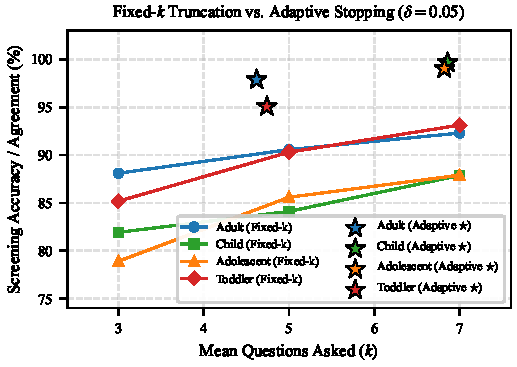
\includegraphics[width=\columnwidth]{fig1_shortening_and_adaptive.pdf}
\caption{Lines: fixed-$k$; stars: adaptive stopping. Accuracy as a function of mean items asked for all cohorts.}
\label{fig:shortening_adaptive}
\vspace{-2mm}
\end{figure}

\subsection{Formulation and Stopping Bounds}
Let $\mathcal{O}_m \subset \{1, \dots, 10\}$ denote the set of items answered at step $m$, and $\mathcal{U}_m = \{1, \dots, 10\} \setminus \mathcal{O}_m$ the unasked items. The posterior probability of screening positive given current responses is $P(Y=1 \mid \mathcal{O}_m)$. At each step, the next item $j^* \in \mathcal{U}_m$ is selected to maximize mutual information with the target label:
\begin{equation}
    j^* = \arg\max_{j \in \mathcal{U}_m} I(Y; A_j \mid \mathcal{O}_m).
\end{equation}

Sequential asking terminates as soon as either of two stopping criteria is met:
\begin{enumerate}
    \item \textbf{Posterior Certainty}: $P(Y=1 \mid \mathcal{O}_m) \ge 1 - \delta$ or $P(Y=1 \mid \mathcal{O}_m) \le \delta$, where $\delta \in (0, 0.5)$ is a clinical confidence parameter.
    \item \textbf{Deterministic Score Bound}: Cumulative score $\sum_{i \in \mathcal{O}_m} A_i \ge t$ (positive triage certain), or $\sum_{i \in \mathcal{O}_m} A_i + |\mathcal{U}_m| < t$ (positive triage impossible).
\end{enumerate}

\begin{table}[t]
\centering
\caption{Adaptive Bayesian Information-Gain Stopping ($\delta=0.05$, Target $95\%$ Certainty)}
\label{tab:adaptive_screener}
\footnotesize
\setlength{\tabcolsep}{3pt}
\resizebox{\columnwidth}{!}{%
\begin{tabular*}{\linewidth}{|@{\extracolsep{\fill}}l|c|c|c|c|c|}
\hline
\textbf{Cohort} & $N$ & $t^*$ & \textbf{Items} & \textbf{Red. \%} & \textbf{Agr. \%} \\
\hline
Adult & 704 & 7 & 4.62 & 53.8\% & 97.87\% \\
\hline
Child & 292 & 7 & 6.86 & 31.4\% & 99.66\% \\
\hline
Adolescent & 104 & 7 & 6.82 & 31.8\% & 99.04\% \\
\hline
Toddler & 1054 & 4 & 4.74 & 52.6\% & 95.07\% \\
\hline
\end{tabular*}}
\vspace{-2mm}
\end{table}

\subsection{Empirical Stopping Results}
As documented in Table~\ref{tab:adaptive_screener}, dynamic Bayesian selection substantially curtails questionnaire length across all age brackets (31.4\%--53.8\% reduction). In the adult cohort, adaptive stopping reaches 97.87\% agreement using an average of just 4.62 items (a 53.8\% workload savings). Toddler assessments yield 95.07\% concordance while cutting average length to 4.74 questions (52.6\% savings). Child (99.66\% agreement, 6.86 mean questions, 31.4\% savings) and adolescent cohorts (99.04\% agreement, 6.82 mean questions, 31.8\% savings) likewise retain high fidelity while sparing families redundant survey items.


\begin{table*}[t]
\centering
\caption{Split Conformal Abstention under Clinical Risk with 100 Repeated $60/20/20$ Splits ($\alpha \in \{0.05, 0.10, 0.20\}$)}
\label{tab:conformal_abstention}
\footnotesize
\setlength{\tabcolsep}{3pt}
\begin{tabular*}{\textwidth}{|@{\extracolsep{\fill}}l|c|c|c|c|c|}
\hline
\textbf{Cohort} & $\alpha$ & \textbf{Nominal Target} & \textbf{Empirical Coverage (Mean $\pm$ SD)} & \textbf{Abstention Rate (Mean $\pm$ SD)} & \textbf{Selective Accuracy (Mean $\pm$ SD)} \\
\hline
Adult & 0.05 & 95\% & 95.74\% $\pm$ 2.78\% & 17.94\% $\pm$ 8.61\% & 95.01\% $\pm$ 2.92\% \\
\hline
Adult & 0.10 & 90\% & 90.61\% $\pm$ 3.39\% & 4.00\% $\pm$ 3.36\% & 91.67\% $\pm$ 2.37\% \\
\hline
Adult & 0.20 & 80\% & 81.86\% $\pm$ 4.34\% & 13.16\% $\pm$ 4.91\% & 94.31\% $\pm$ 2.21\% \\
\hline
Child & 0.05 & 95\% & 96.68\% $\pm$ 3.46\% & 37.61\% $\pm$ 22.46\% & 95.42\% $\pm$ 4.21\% \\
\hline
Child & 0.10 & 90\% & 91.85\% $\pm$ 5.17\% & 14.20\% $\pm$ 8.56\% & 91.00\% $\pm$ 5.20\% \\
\hline
Child & 0.20 & 80\% & 80.78\% $\pm$ 7.13\% & 9.97\% $\pm$ 8.88\% & 89.25\% $\pm$ 4.72\% \\
\hline
Adolescent & 0.05 & 95\% & 95.62\% $\pm$ 5.86\% & 55.29\% $\pm$ 28.85\% & 93.26\% $\pm$ 8.36\% \\
\hline
Adolescent & 0.10 & 90\% & 91.33\% $\pm$ 7.26\% & 28.14\% $\pm$ 23.69\% & 89.75\% $\pm$ 7.49\% \\
\hline
Adolescent & 0.20 & 80\% & 82.62\% $\pm$ 10.20\% & 11.48\% $\pm$ 9.83\% & 87.18\% $\pm$ 7.24\% \\
\hline
Toddler & 0.05 & 95\% & 95.35\% $\pm$ 1.96\% & 14.94\% $\pm$ 5.79\% & 94.60\% $\pm$ 2.03\% \\
\hline
Toddler & 0.10 & 90\% & 90.91\% $\pm$ 2.71\% & 2.91\% $\pm$ 2.38\% & 92.02\% $\pm$ 1.92\% \\
\hline
Toddler & 0.20 & 80\% & 81.46\% $\pm$ 3.80\% & 13.75\% $\pm$ 3.88\% & 94.46\% $\pm$ 1.55\% \\
\hline
\end{tabular*}
\vspace{-2mm}
\end{table*}

\section{Conformal Abstention Under Clinical Risk}

These classification models force a binary decision on each case, even when model confidence is restricted to $P \approx 0.50$ (50\%). Making arbitrary binary guesses in medical triage can create dangerous false reassurance. We have used split-conformal prediction~\cite{vovk2005algorithmic, angelopoulos2021gentle} to supply marginal coverage under exchangeability. into 3 distinct parts (60\% training, 20\% calibration and 20\% evaluation). Separating calibration data from training data eliminates overconfidence altogether.

\begin{figure}[t]
\centering
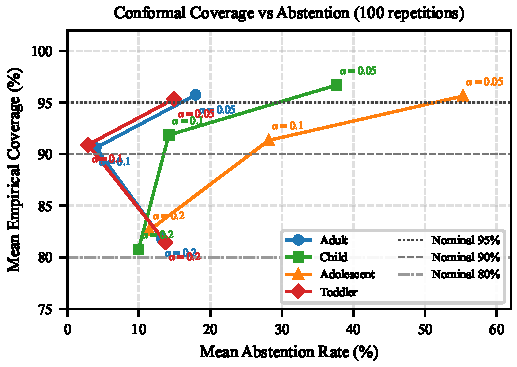
\includegraphics[width=\columnwidth]{fig2_conformal_abstention.pdf}
\caption{The coverage vs. abstention trade-off at different error levels $\alpha \in \{0.05, 0.10, 0.20\}$ using held-out calibration.}
\label{fig:conformal_tradeoff}
\vspace{-2mm}
\end{figure}

\subsection{Split Conformal Calibration}

For each calibration case $(X_i, Y_i)$ its non-conformity score is defined as $s_i = 1 - \hat{P}(Y_i \mid X_i)$. For a targeted error budget $\alpha \in (0, 1)$, we calculate empirical quantile $\hat{q}$:
\begin{equation}
    \hat{q} = \text{Quantile}\left(\{s_i\}_{i=1}^n, \frac{\lceil(n+1)(1-\alpha)\rceil}{n}\right).
\end{equation}
For each test instance $X$, the conformal prediction set is constructed as:
\begin{equation}
    C(X) = \{y \in \{0, 1\} : 1 - \hat{P}(y \mid X) \le \hat{q}\}.
\end{equation}
If $C(X) = \{1\}$ the screener suggests a high priority referral; $C(X) = \{0\}$ suggests a low likelihood. When $C(X) = \{0, 1\}$, the confidence is not sufficient to discriminate between the outcomes and an automated abstention is made: \textit{``Specialist Assessment Required''}.

\subsection{Empirical Coverage and Abstention Dynamics}

Table~\ref{tab:conformal_abstention} and Fig.~\ref{fig:conformal_tradeoff} show calibration metrics averaged over 100 randomly seeded 60/20/20 train/calibration/test splits. For $\alpha=0.05$ ($95\%$ target coverage), the empirical coverage is in good agreement with theoretical thresholds: $95.35\% \pm 1.96\%$ for toddlers, $96.68\% \pm 3.46\%$ for children, $95.62\% \pm 5.86\%$ for adolescents and $95.74\% \pm 2.78\%$ for adults. At $\alpha = 0.10$, coverage averages $90.61\% \pm 3.39\%$ in adults, $90.91\% \pm 2.71\%$ in toddlers, $91.33\% \pm 7.26\%$ in adolescents, and $91.85\% \pm 5.17\%$ in children. At $\alpha = 0.20$, coverage remains well-aligned ($80.78\% \pm 7.13\%$ to $82.62\% \pm 10.20\%$). Occasional empty prediction sets that occur when calibration quantiles fall below 0.50 at $\alpha = 0.20$ are conservatively routed to the abstention pool. We validate conformal triage as a principled mechanism for clinical risk escalation, with selective accuracy reaching 94.60\% $\pm$ 2.03\% for toddlers and 95.01\% $\pm$ 2.92\% for adults at $\alpha = 0.05$ amongst retained singleton decisions.

\section{Negative Audit: Open Facial Image Benchmark}

Several recent studies report that deep convolutional networks can detect autism from face photos in the open Autism Image Data benchmark~\cite{senol2020autism}. While papers cite 2,940 images, the dataset contains 3,014 photographs (1,507 autistic, 1,507 neurotypical). We investigated this benchmark for test set leakage, photographic confounders, and shortcut learning.

\begin{figure}[t]
\centering
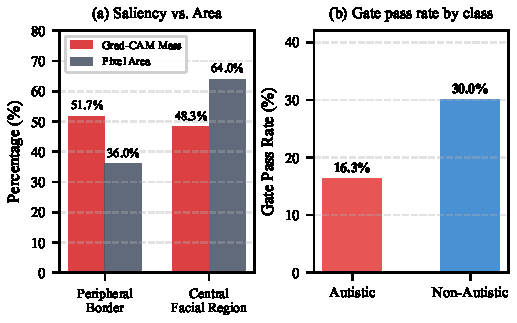
\includegraphics[width=\columnwidth]{fig3_gradcam_shortcut.pdf}
\caption{Audit of paediatric face benchmark: (a) Visual attribution mass (via Grad-CAM) focused on the border areas of the image relative to a baseline physical area; (b) Per-class systematic quality gate pass rate differential ($p = 5.44 \times 10^{-19}$).}
\label{fig:face_audit_fig}
\vspace{-2mm}
\end{figure}

\subsection{Acquisition Disparities and Quality Gate Auditing}

We passed all 3,014 photographs through automated facial quality checks (BlazeFace detector and 468-point MediaPipe mesh) using production filtering criteria: head yaw $\le 15^\circ$, head pitch $\le 15^\circ$, iris asymmetry $\le 12\%$, Laplacian blur variance $\ge 100$, and iris diameter $\ge 22\,\text{px}$.

\begin{table}[t]
\centering
\caption{Negative Audit for Open Pediatric Face Benchmark (Autism Image Data, $N = 3{,}014$)}
\label{tab:face_audit}
\footnotesize
\setlength{\tabcolsep}{3pt}
\resizebox{\columnwidth}{!}{
\begin{tabular}{|p{0.55\columnwidth}|p{0.35\columnwidth}|}
\hline
\textbf{Audit Dimension / Failure Mode} & \textbf{Empirical Metric} \\
\hline
Cross-Split Contamination (Valid vs. Test MD5) & 56 duplicate pairs (split leakage) \\
\hline
Perceptual Duplication (Hamming Distance $\le 4$) & no additional beyond exact matches \\
\hline
Quality Gate Pass Rate Discrepancy & 16.32\% aut. vs. 29.99\% non-aut. ($p < 10^{-18}$) \\
\hline
Peripheral Illumination Discrepancy ($\Delta L$) & 7.72 pixel intensity units (0--255) \\
\hline
Grad-CAM Saliency Energy in 10\% Outer Border & 51.73\% (physical area baseline: 36.00\%) \\
\hline
Retrained MobileNetV2 Accuracy (Clean Split) & 49.55\% (Chance level: $50.00\%$, AUC: 0.4595) \\
\hline
\end{tabular}
}
\vspace{-2mm}
\end{table}

Initial face detection succeeded across all benchmark photographs ($0/1{,}507$ failed detection, $100.00\%$ raw face detection rate), but strict quality gate pass rates revealed stark differences: only $16.32\%$ ($246/1{,}507$) of autistic photos passed all five checks, compared to $29.99\%$ ($452/1{,}507$) of control images ($\chi^2 = 78.35, p = 8.62 \times 10^{-19}$; Fisher's exact $p = 5.44 \times 10^{-19}$, odds ratio $0.455$). Control portraits featured larger irises (median $23.13$ vs. $18.82$ px, Mann-Whitney $p = 8.38 \times 10^{-25}$), better image sharpness ($296.44$ vs. $232.48$, $p = 3.39 \times 10^{-6}$), and straighter head alignment ($4.80^\circ$ vs. $6.10^\circ$, $p = 1.16 \times 10^{-6}$). These systematic photography differences show that vision models learn dataset collection flaws rather than autism phenotypes.

\subsection{Grad-CAM Visual Attribution and Shortcut Verification}

To see what image features guide predictions, we trained MobileNetV2~\cite{sandler2018mobilenetv2} on the dataset and extracted Grad-CAM heatmaps~\cite{selvaraju2017grad}. Fig.~\ref{fig:face_audit_fig} maps the resulting attribution density. The image border that is outer 10\% contains 51.73\% of the total saliency energy, despite being just 36.00\% of the overall image area. Instead of focusing on landmarks of the eyes, nose, or mouth, lighting, framing, and compression artifacts along the perimeter are factors the model relies on. As convolutional networks trained on this dataset learn photographic shortcuts rather than clinical features~\cite{geirhos2020shortcut}, models from facial images need to be omitted from diagnostic screening instruments and limited to auditing image quality.

\section{Discussion, Limitations, and Conclusion}

\subsection{Discussion}
Machine learning in healthcare demands rigorous audits of base data collected. Reported accuracy across autism survey benchmark tests ranging from 98\% to 100\% reflects memorization of fixed addition thresholds ($t = 4$ for toddlers; $t = 7$ for the older cohorts), rather than medical discovery. Meanwhile, camera framing and quality artifacts are being exploited by facial vision models rather than neurodevelopmental phenotypes. Computational methods provide genuine clinical utility when reformulated for triage: dynamic item selection reduces caregiver burden by 31.4\% to 53.8\% while preserving fidelity, and split-conformal prediction is valid under exchangeability, routing ambiguous cases to the appropriate specialist.

\subsection{Limitations}
There are a number of limitations to our findings. First, open survey data sets are retrospective volunteer submissions, not balanced prospective populations. Second, conformal marginal coverage relies on data exchangeability; at $\alpha = 0.05$, for children, the average abstention is 37.6\% and for adolescents it is 55.3\%, requiring adequate specialized referral capacity. Third, face benchmarks from online sources are substantially different than controlled clinical photography. Finally, verifying physical camera distance needs a minimum of 20 calibration ID-1 card images.

\subsection{Conclusion}
Machine learning cannot, and should not, fill the role of comprehensive neurodevelopmental assessments by clinical experts. But, by honest questionnaire shortening, shortcut auditing, and marginal coverage within the limits of exchangeability, computational screening can support early developmental triage.

\section*{Data and Code Availability}
You can find the code and result files from the authors on request.

\section*{Acknowledgment}
The authors recognize the utilization of research infrastructure and institutional support at Vel Tech Rangarajan Dr. Sagunthala R\&D Institute of Science and Technology. All conceptual formulations, statistical analyses, experimental audits, and manuscript interpretations were carefully screened and checked by the authors.

\begin{thebibliography}{16}
\footnotesize
\setlength{\itemsep}{0pt}
\setlength{\parskip}{0pt}
\footnotesize
\setlength{\itemsep}{1pt}

\bibitem{american2013diagnostic}

American Psychiatric Association, \emph{Diagnostic and Statistical Manual of Mental Disorders}, 5th~ed.\hskip 1em plus 0.5em minus 0.4em\relax Arlington, VA: American Psychiatric Publishing, 2013. doi: 10.1176/appi.books.9780890425596.

\bibitem{allison2012toward}

C.~Allison, B.~Auyeung, and S.~Baron-Cohen, ``Toward Brief ``Red Flags'' for Autism Screening: The Short Autism Spectrum Quotient and the Short Quantitative Checklist in 1,000 Cases and 3,000 Controls,'' \emph{Journal of the American Academy of Child \& Adolescent Psychiatry}, vol.~51, no.~2, pp. 202--212, 2012. doi: 10.1016/j.jaac.2011.11.003.

\bibitem{thabtah2017autism}

F.~Thabtah, ``Autism Spectrum Disorder Screening: Machine Learning Adaptation and DSM-5 Fulfillment,'' in \emph{Proceedings of the 1st International Conference on Medical and Health Informatics (ICMHI 2017)}, 2017, pp. 1--6. doi: 10.1145/3107514.3107515.

\bibitem{thabtah2018qchat}

F.~Thabtah, F.~Kamalov, and K.~Rajab, ``A new computational intelligence approach to detect autistic features for autism screening,'' \emph{International Journal of Medical Informatics}, vol.~117, pp. 112--124, 2018. doi: 10.1016/j.ijmedinf.2018.06.009.

\bibitem{thabtah2019machine}

F.~Thabtah, ``Machine learning in autistic spectrum disorder behavioral research: A review and ways forward,'' \emph{Informatics for Health and Social Care}, vol.~44, no.~3, pp. 278--297, 2019. doi: 10.1080/17538157.2017.1399132.

\bibitem{senol2020autism}

C.~Senol, ``Autism Image Data,'' \emph{Kaggle}, 2020. [Online]. Available: \url{https://www.kaggle.com/datasets/cihan063/autism-image-data}.

\bibitem{kapoor2023leakage}

S.~Kapoor and A.~Narayanan, ``Leakage and the reproducibility crisis in machine-learning-based science,'' \emph{Patterns}, vol.~4, no.~9, p. 100804, 2023. doi: 10.1016/j.patter.2023.100804.

\bibitem{geirhos2020shortcut}

R.~Geirhos, J.-H. Jacobsen, C.~Michaelis, R.~Zemel, W.~Brendel, M.~Bethge, and F.~A. Wichmann, ``Shortcut learning in deep neural networks,'' \emph{Nature Machine Intelligence}, vol.~2, no.~11, pp. 665--673, 2020. doi: 10.1038/s42256-020-00257-z.

\bibitem{sandler2018mobilenetv2}

M.~Sandler, A.~Howard, M.~Zhu, A.~Zhmoginov, and L.-C. Chen, ``MobileNetV2: Inverted residuals and linear bottlenecks,'' in \emph{IEEE/CVF Conference on Computer Vision and Pattern Recognition (CVPR)}, 2018, pp. 4510--4520. doi: 10.1109/CVPR.2018.00474.

\bibitem{selvaraju2017grad}

R.~R. Selvaraju, M.~Cogswell, A.~Das, R.~Vedantam, D.~Parikh, and D.~Batra, ``Grad-CAM: Visual explanations from deep networks via gradient-based localization,'' in \emph{IEEE International Conference on Computer Vision (ICCV)}, 2017, pp. 618--626. doi: 10.1109/ICCV.2017.74.

\bibitem{vovk2005algorithmic}

V.~Vovk, A.~Gammerman, and G.~Shafer, \emph{Algorithmic Learning in a Random World}.\hskip 1em plus 0.5em minus 0.4em\relax New York: Springer, 2005. doi: 10.1007/b106715.

\bibitem{angelopoulos2021gentle}

A.~N. Angelopoulos and S.~Bates, ``A gentle introduction to conformal prediction and distribution-free uncertainty quantification,'' \emph{arXiv preprint arXiv:2107.07511}, 2021. doi: 10.48550/arXiv.2107.07511.

\bibitem{uci_asd_adult}
F.~Thabtah, ``Autism Screening Adult,'' \emph{UCI Machine Learning Repository}, 2017. [Online]. Available: \url{https://archive.ics.uci.edu/dataset/426}.

\bibitem{uci_asd_child}
F.~Thabtah, ``Autism Screening Child,'' \emph{UCI Machine Learning Repository}, 2017. [Online]. Available: \url{https://archive.ics.uci.edu/dataset/419}.

\bibitem{uci_asd_adolescent}
F.~Thabtah, ``Autism Screening Adolescent,'' \emph{UCI Machine Learning Repository}, 2017. [Online]. Available: \url{https://archive.ics.uci.edu/dataset/420}.

\bibitem{kaggle_toddler}
F.~Fayez, ``Autism Screening for Toddlers,'' \emph{Kaggle}, 2018. [Online]. Available: \url{https://www.kaggle.com/datasets/fabdelja/autism-screening-for-toddlers}.

\end{thebibliography}

\end{document}

